\documentclass[12pt, a4paper]{article}

\usepackage{graphicx}
\usepackage{float}
\usepackage{hyperref}


\begin{document}

\section{Theoretical Background}

	\subsection{Modulator}
	\subsection{Demodulator Circuit}
		A demodulator circuit is one of the applications of a diode as a detector for amplitude modulated (AM) radio signals. An AM signal consists of a radio-frequency carrier wave whose amplitude varies with different audio frequencies.

		The detector circuit circuit is essentially a half-wave rectifier circuit with an RC filter placed on the output as can be seen from the circuit of the modulator cicruit for this practical in Figure \ref{demodulator_circuit}.

		The RC time constant of the fitler should fall between 2 values
		\begin{equation}
			\frac{1}{\omega_c} \le RC \le \frac{\sqrt{1-\mu^2}}{\omega_m\mu}
		\end{equation}

		where $\omega_c$ is the frequency of the carrier, $\omega_m$ is the angular frequency of the information and $\mu$ is the modulation index

		This result comes from practical experience in the field of electronic engineering rather than from a mathematical principles.

		If the $RC$ time constant is to small, there would be ripples of the carrier frequency on the ouput (this is to be avoided as we require the information sent rather than the disotrtion thereof with the carrier signal).

		If the $RC$ time constant is to big, it will significantly attenuate high frequencies 


		\begin{figure}[H]
			\centering
			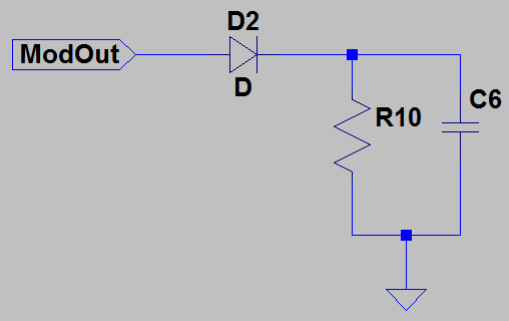
\includegraphics[width=0.7\textwidth]{images/Demodulator_circuit.png}
			\caption{The demodulator circuit used for this experiment}
			\label{demodulator_circuit}
		\end{figure}

	\subsection{}



\begin{thebibliography}{9}

	\bibitem{lamport94}
	  Donald A. Neamen,
	  \textit{Microelectronics: Circuit Analysis and Design}

	\bibitem{Detector}
	Phil Frost
	\textit{RC time constant and diode detector}
	\texttt{https://electronics.stackexchange.com/questions/100518/rc-time-constant-and-diode-detector}

\end{thebibliography}

\end{document}